%This is my super simple Real Analysis Homework template

\documentclass{article}
\usepackage[]{amsthm} %lets us use \begin{proof}
\usepackage[]{amssymb} %gives us the character \varnothing
\usepackage[T1]{fontenc}
\usepackage[polish]{babel}
\usepackage{listings}
\usepackage{hyperref}
\hypersetup{
    colorlinks=true,
    linkcolor=blue,
    filecolor=magenta,      
    urlcolor=cyan,
}
\usepackage{graphicx}
\graphicspath{ {./ryciny/} }
\usepackage{caption}
\usepackage{subcaption}

\title{Testowanie algorytmu Quick Sort}
\author{Konrad Pagacz gr. 21}
\date\today
%This information doesn't actually show up on your document unless you use the maketitle command below

\usepackage{geometry}
\geometry{
legalpaper,
margin=2cm
}

\begin{document}
\maketitle %This command prints the title based on information entered above

\section{Środowisko}
Postanowiłem zaimplementować algorytmy w języku C++.

\section{Analiza warunków początkowych zadania}
Zadanie żąda, by tablice były o rozmiarach do 1 000 000 elementów i by elementy przynajmniej w jednym sposobie były losowane do tablicy z zakresu większego niż jej rozmiar, czyli większego niż 1 000 000. To oznacza, że wystarczy deklarować tablicę typu \textit{int}, ponieważ typ ten pomieści elementy aż do wartości 2 147 483 647, czyli zdecydowanie ponad to, co wymagane jest w zadaniu. 

\section{Opis implementacji}
    \subsection{Funkcja sortująca z optymalizacjami - głowne wyniki}
    Zaimplementowałem sortowanie Quick Sort. Jako sposób partycji wybrałem partycję sposobem Lomuto. Wprowadziłem dwie optymalizacje do algorytmu sortującego:
    \begin{itemize}
        \item {Zamiast dwóch rekursywnych wywołań funkcji sortującej w ciele funkcji sortującej, wykonuję jedno wywołanie funkcji partycji (determinujące element osiowy), a następnie jedno wywołanie rekursywne na mniejszej części tablicy przedzielonej elementem osiowym (tzw. \textit{tail recursion}).}
        \item {Funkcja dokonująca partycji grupuje elementy równe elementowi osiowemu obok siebie oraz zwraca dwie wartości zamiast jednej - pierwsza wskazująca indeks pierwszego elementu równego elementowi osiowemu oraz druga wskazująca indeks ostatniego elementu równego elementowi osiowemu.}
    \end{itemize}
    
    \subsection{Funkcja sortująca bez optymalizacji - dodatkowe wyniki}
    Zdecydowałem się też w celach pokazania różnic pomiędzy zoptymalizowanym i niezoptymalizowanym Quick Sortem zaimplementować Quick Sort z partycją sposobem Lomuto, ale bez żadnych optymalizacji, czyli algorytm zaprezentowany w trakcie wykładu. Ze względu na bardzo długi czas wykonywania się algorytmów dla dużych rozmiarów tablic, ograniczyłem rozmiar tablicy dla eksperymentów z funkcją bez optymalizacji do 50 tysięcy elementów.
    
    \subsection{Znajdowanie mediany}
    Znajdowałem medianę pierwszych 3, 5 lub 7 elementów tablicy. Do znalezienia mediany korzystałem z zaimplementowanej przeze mnie funkcji QuickSelect.

\section{Sposób generowania danych}
    \subsection{Generator liczb pseudolosowych}
    Zdecydowałem się użyć rekomendowanego przez \url{https://en.cppreference.com/w/cpp/numeric/random} sposobu generowania liczb pseudolosowych. Wykorzystałem funkcję losowanie liczb z rozkładu jednorodnego wraz z generatorem liczb pseudolosowych Mersenne Twister opisanym przez Matsumoto i Nishimurę w 1998 umieszczone w bibliotece \textit{random}.
    
    \subsection{Generowanie danych a pojedynczy eksperyment}
    Każdy eksperyment składający się z posortowania tablicy o określonym rozmiarze, wypełnionej elementami w określony sposób i przy wyborze elementu osiowego w konkretny sposób korzystał z danych wygenerowanych tylko na jego potrzeby. Żadne raz wygenerowane tablice nie były używane w kolejnych eksperymentach.
    
    \subsection{Wypełnianie tablicy elementami pseudolosowymi z zakresu przekraczającego rozmiar tablicy}
    Losowałem elementy z rozkładu jednorodnego z zakresu \(0\) do \(2 * rozmiar\).
    
    \subsection{Wypełnianie tablicy elementatmi pseudolosowymi z zakresu od 0 do 100}
    Losowałem elementy z rozkładu jednorodnego z zakresu od \(0\) do \(100\).
    
    \subsection{Wypełnianie tablicy elementami uporządkowanymi niemalejąco}
    Wypełnilem tablicę w następujący sposób: element tablicy o indeksie \(i\) miał wartość \(i\).
    
\section{Pomiar czasu}
Mierzyłem czas przy pomocy biblioteki \textit{ctime} i funkcji \textit{std::clock()}. Zmierzony czas był tylko czasem sortowania z dokładnością do milisekundy. Zależało mi, by zmierzyć faktyczny czas pracy procesora, a nie czas, który upłynął w rzeczywistości, stąd też wybór tejże biblioteki. Ma ona swoje wady, między innymi nie mierzy czasu procesora poświęconego w programach wykorzystujących wiele wątków procesora, natomiast żadna z nich nie miała wpływu na wyniki mojego jednowątkowego programu.

\section{Wyniki}
    \subsection{Quick Sort z optymalizacjami - główne wyniki}
    Podzieliłem główne wyniki na trzy sekcje, każda odpowiadająca jednemu sposobowi wypełniania tablicy elementami.
        \subsubsection{Wypełnianie elementami losowymi z zakresu przekraczającego rozmiar tablicy}
        Czas sortowania był najszybszy, gdy element osiowy był wybierany jako pierwszy lub ostatni element (rysunek \ref{fig:optimized:random_fill}). Dla 10000 elementów najszybszy był wybór elementu ostatniego (0,011 s) tak samo jak dla 1000000 (1,780 s). Sortowanie postępowało najwolniej przy wyborze elementu osiowego jako mediany pierwszych 7 elementów tablicy wejściowej.
        \begin{figure}
            \centering
            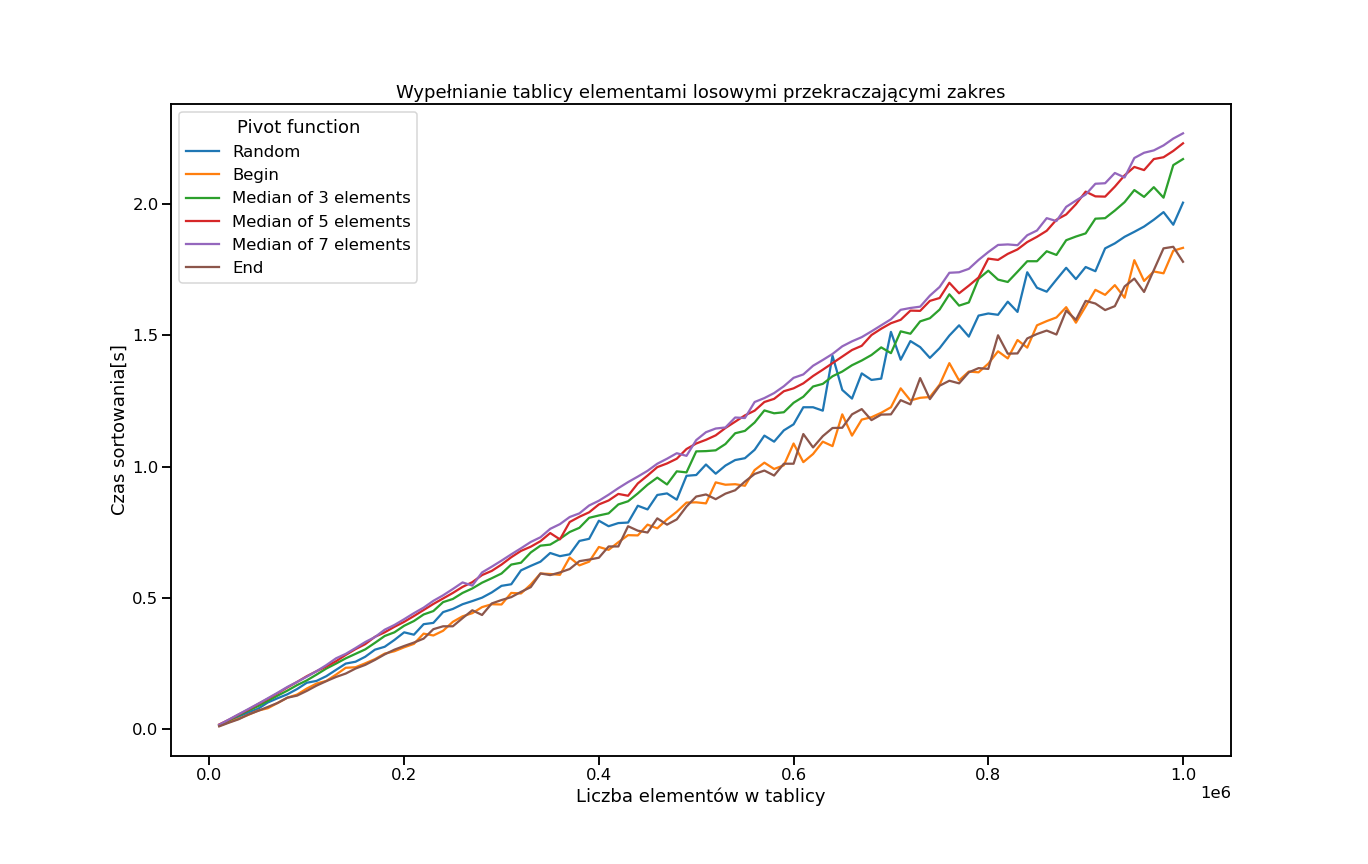
\includegraphics[width=\textwidth]{ryciny/optymalizacje/lineplot-random-fill.png}
            \caption{Czas działania zoptymalizowanego algorytmu sortującego w zależności od liczby elementów w tablicy. Elementy tablicy były wstawiane zgodnie z rozkładem jednorodnym z zakresu od 0 do podwojonego rozmiaru tablicy.}
            \label{fig:optimized:random_fill}
        \end{figure}
        
        \subsubsection{Wypełnianie elementami losowymi z zakresu od 0 do 100}
        Czas sortowania wahał się od 0,004 sekundy do 0,549 sekundy (rysunek \ref{fig:optimized:100_fill}). Czas sortowania był najszybszy, gdy element osiowy był wybierany jako mediana pierwszych kilku elementów.
        \begin{figure}
            \centering
            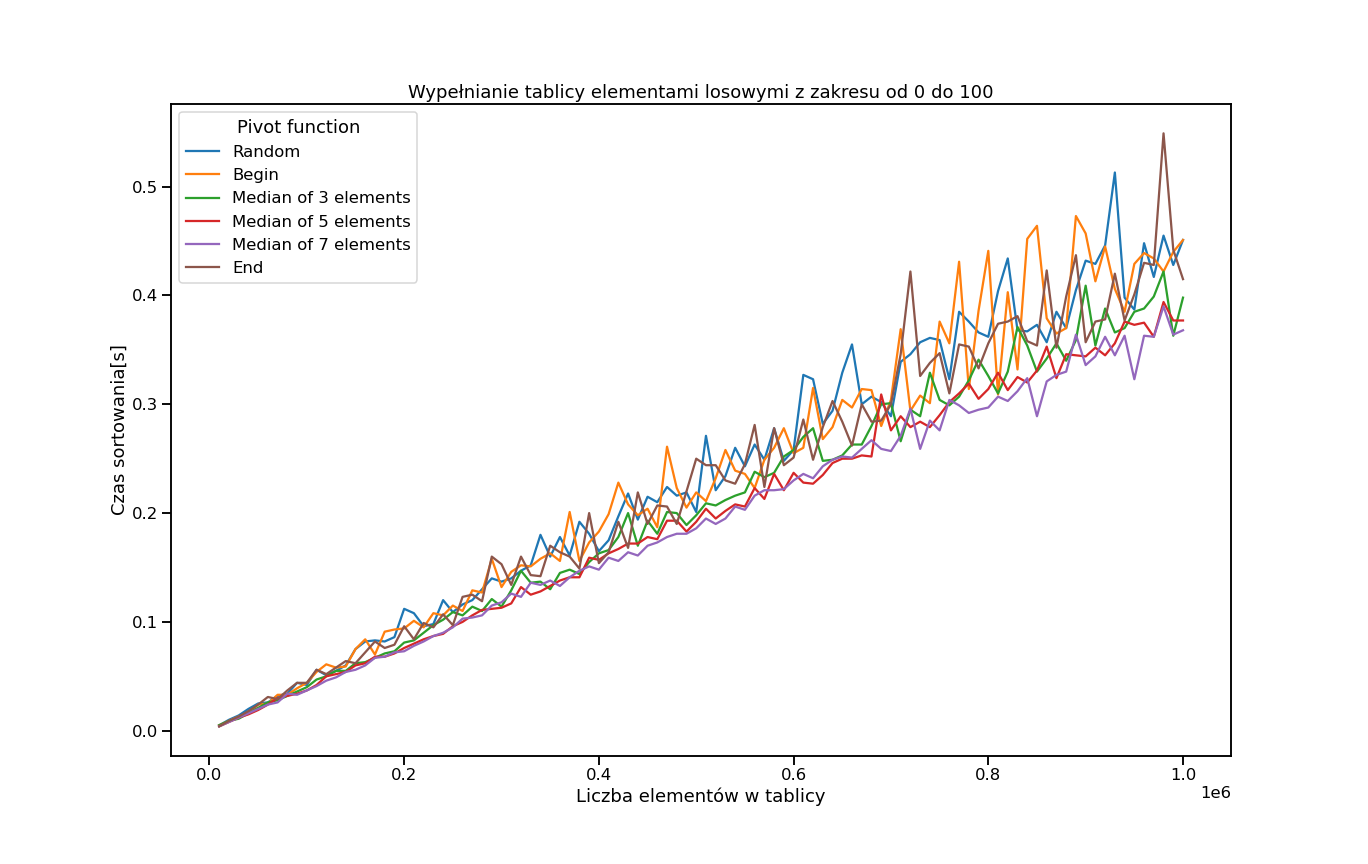
\includegraphics[width=\textwidth]{ryciny/optymalizacje/lineplot-100-fill.png}
            \caption{Czas działania zoptymalizowanego algorytmu sortującego w zależności od liczby elementów w tablicy. Elementy tablicy były wstawiane zgodnie z rozkładem jednorodnym z zakresu od 0 do 100.}
            \label{fig:optimized:100_fill}
        \end{figure}
        
        \subsubsection{Wypełnianie elementami w sposób niemalejący}
        Czas sortowania wahał się od 0,015 s do 2530,168 s (rysunek \ref{fig:optimized:nondecreasing_fill}). Dla wyboru elementu osiowego jako ostatniego elementu tablicy wejściowej wyniki są kompletne tylko do rozmiaru tablicy równemu 280000 elementów. Algorytm sortujący działał najdłużej przy wyborze ostatniego elementu tablicy jako elementu osiowego, zdecydowanie wolniej od innych działał również przy wyborze pierwszego elementu tablicy jako elementu osiowego.
        \begin{figure}
            \centering
            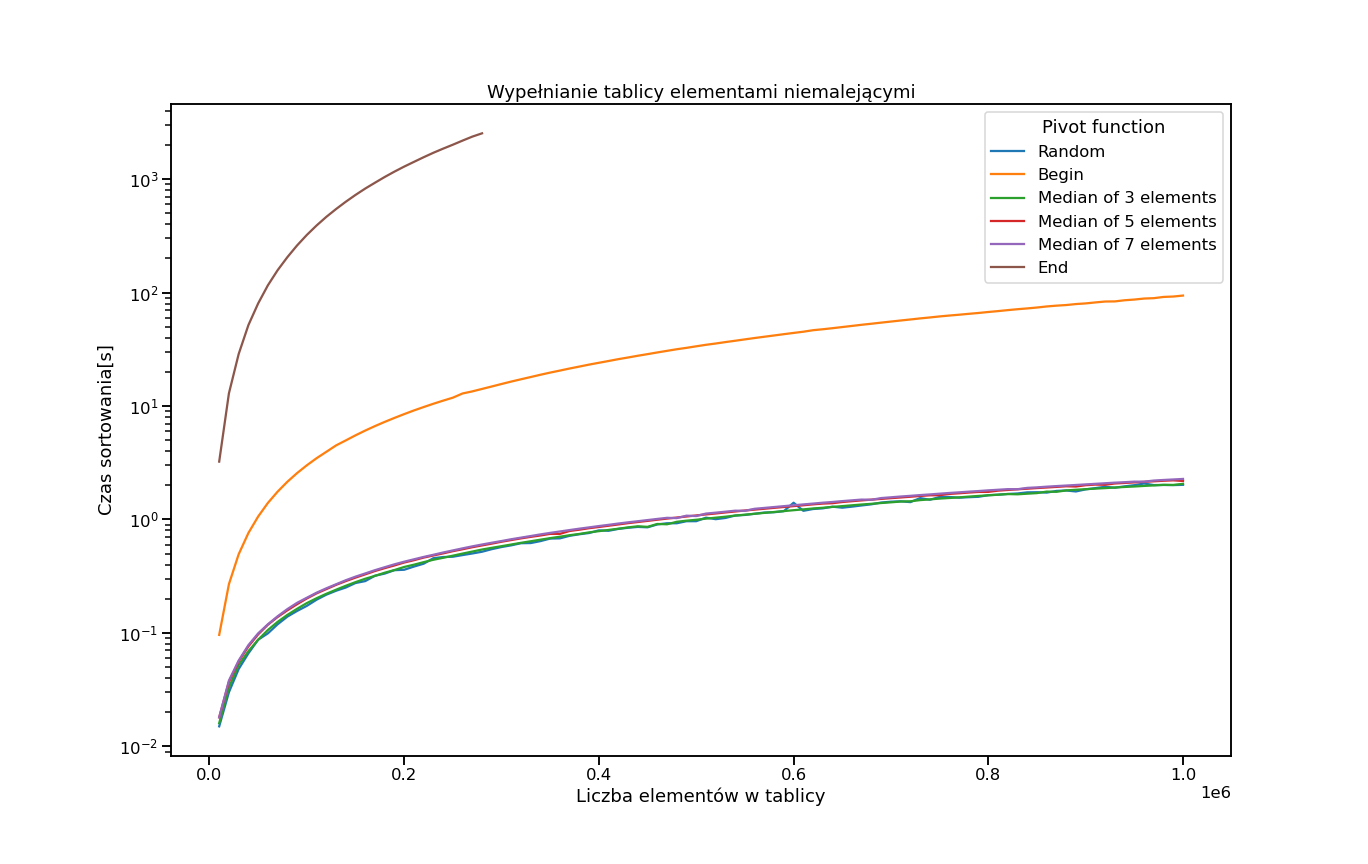
\includegraphics[width=\textwidth]{ryciny/optymalizacje/lineplot-nondecreasing-fill-log-scale.png}
            \caption{Czas działania zoptymalizowanego algorytmu sortującego w zależności od liczby elementów w tablicy. Elementy tablicy były wstawiane w sposób niemalejący.}
            \label{fig:optimized:nondecreasing_fill}
        \end{figure}
    
    \subsection{Quick Sort bez optymalizacji}
    \begin{figure}
        \centering
        \begin{subfigure}[t]{0.47\textwidth}
            \centering
            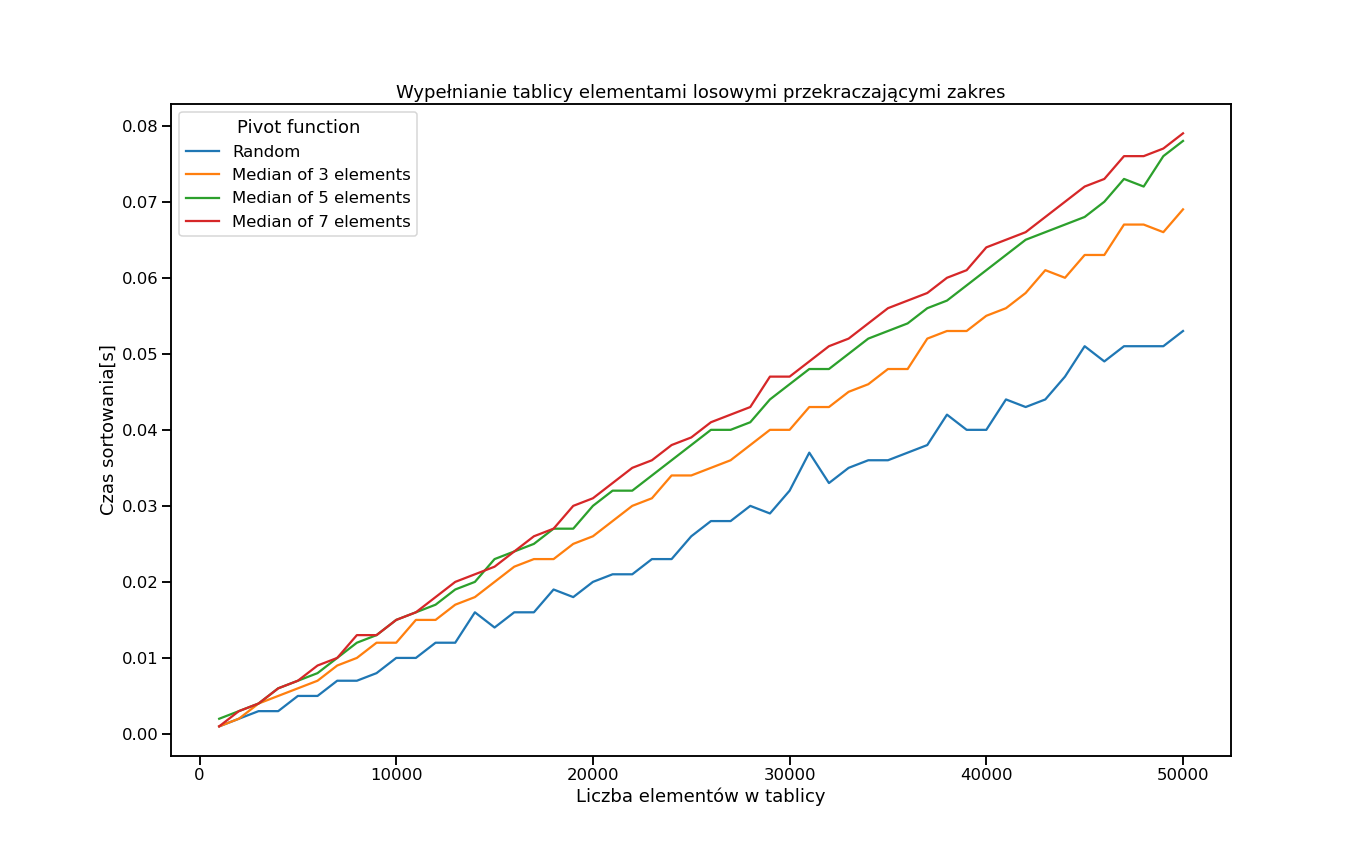
\includegraphics[width=\linewidth]{ryciny/bez-optymalizacji/lineplot-random-fill-unoptimized.png}
            \caption{Czas działania niezoptymalizowanego algorytmu sortującego w zależności od liczby elementów w tablicy. Elementy tablicy były wstawiane zgodnie z rozkładem jednorodnym z zakresu od 0 do podwojonego rozmiaru tablicy.}
            \label{fig:unoptimized:random_fill}
        \end{subfigure}
        \hfill
        \begin{subfigure}[t]{0.47\textwidth}
            \centering
            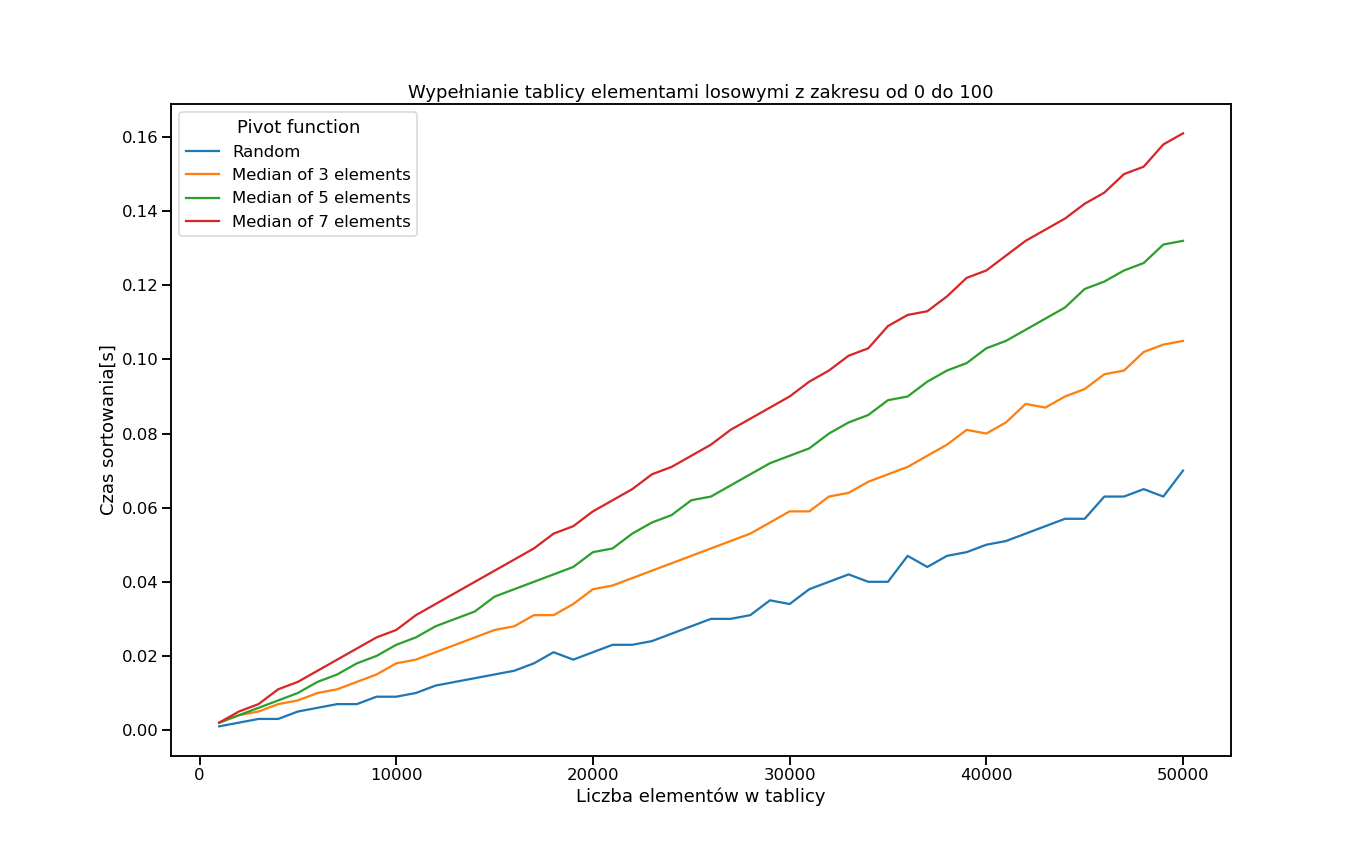
\includegraphics[width=\linewidth]{ryciny/bez-optymalizacji/lineplot-100-fill-unoptimized.png}
            \caption{Czas działania niezoptymalizowanego algorytmu sortującego w zależności od liczby elementów w tablicy. Elementy tablicy były wstawiane zgodnie z rozkładem jednorodnym z zakresu od 0 do 100.}
            \label{fig:unoptimized:100_fill}
        \end{subfigure}
        \newline
        \begin{subfigure}[t]{0.47\textwidth}
            \centering
            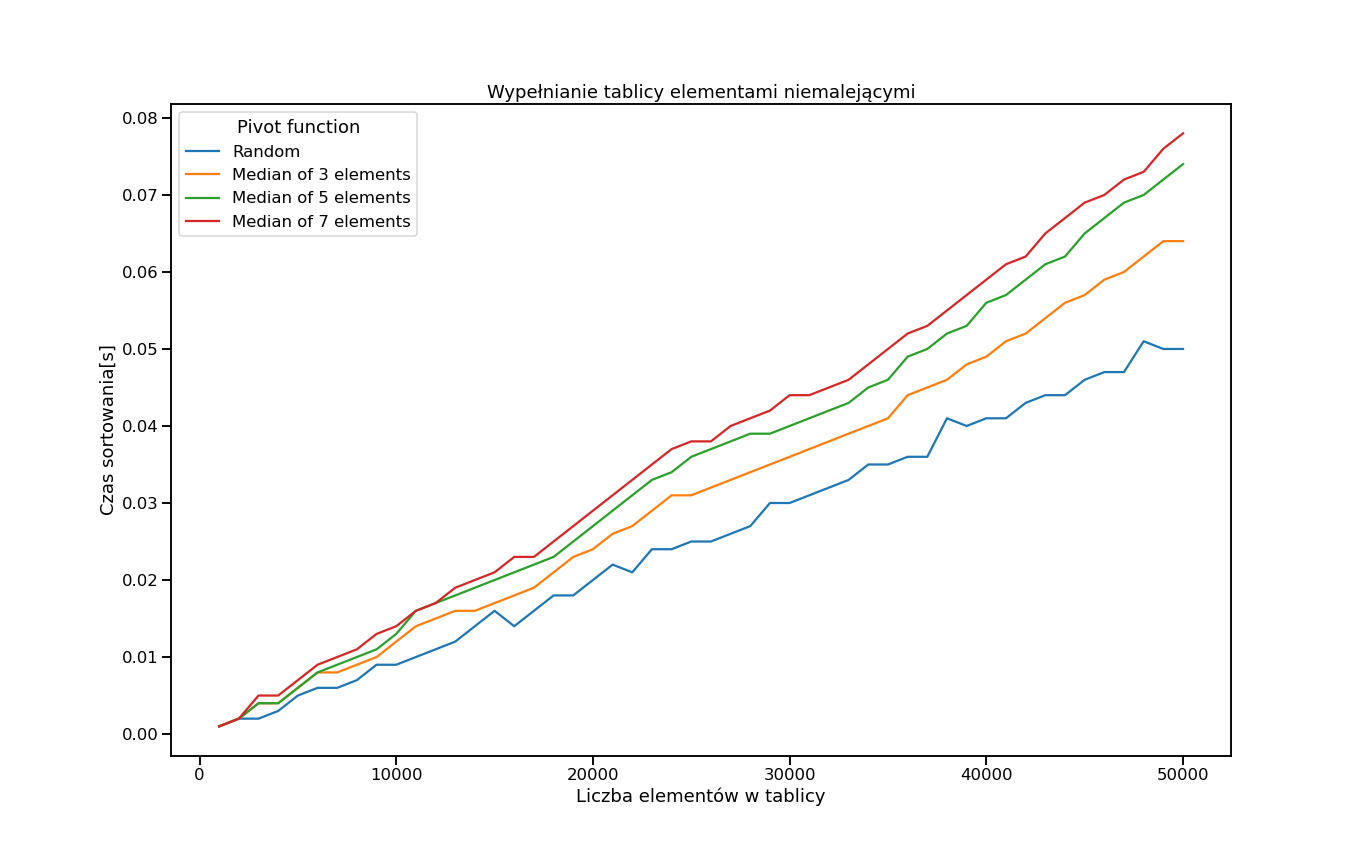
\includegraphics[width=\linewidth]{ryciny/bez-optymalizacji/lineplot-nondecreasing-fill-unoptimized.png}
            \caption{Czas działania niezoptymalizowanego algorytmu sortującego w zależności od liczby elementów w tablicy. Elementy tablicy były wstawiane niemalejąco.}
            \label{fig:unoptimized:nondecreasing_fill}
        \end{subfigure}
        \hfill
        \begin{subfigure}[t]{0.47\textwidth}
            \centering
            \includegraphics[width=\linewidth]{ryciny/bez-optymalizacji/random-vs-100-fill-unoptimized.png}
            \caption{Czas działania niezoptymalizowanego algorytmu sortującego w dwóch metodach wyboru elementu osiowego.}
            \label{fig:unoptimized:rand-vs-100}
        \end{subfigure}
        \caption{Czasy działania niezoptymalizowanego algorytmu sortującego.}
        \label{fig:unoptimized}
    \end{figure}
    Wyniki algorytmu Quick Sort bez optymalizacji znajdują się na rysunku \ref{fig:unoptimized}. Dla liczby elementów powyżej 10 000 wybór pierwszego lub ostatniego elementu osiowego dla wypełnienia tablicy niemalejąco zwracał błąd naruszenia ochrony pamięci.

\section{Dyskusja}
\subsection{Quick Sort z optymalizacjami}
Szybkość sortowania algorytmem Quick Sort jest zależna od charakteru danych wejściowych. Wyniki wskazywały na to, że sortowanie tablicy z dużą liczbą powtarzających się elementów jest najszybsze. Ten wynik jest związany z jedną z optymalizacji - w mojej implementacji algorytm nie sortował ponownie wartości równych elementom osiowym, więc jeśli było ich dużo w tablicy (tak jak w tym przypadku losowania), to sortowanie następowało szybciej niż w przypadku zupełnie różnych wartości elementów tablicy. Najszybsze działanie algorytmu w tym sposobie losowania zaobserwowałem przy wyborze elementu osiowego jako mediany pierwszych 7 elementów, lecz nie potrafię wyjaśnić, czemu metody oparte na medianie w tej metodzie wypełniania tablicy radziły sobie lepiej niż wybór losowy. Przy tej metodzie wypełniania zaobserwowałem również największą zmienność długości trwania algorytmu - zapewne związaną z tym, że dobry wybór elementu osiowego jest kluczowy dla posortowania tablicy wypełnionej małą liczbą, ale wielokrotnie powtórzonych wartości.

Przy wypełnianiu tablicy losowo, najszybsze działanie aglorytmu zapewniał wybór pierwszego lub ostatniego elementu jako osiowy. Wybór elementu losowego lub policzenie mediany jest związane z dodatkowym czasem działania algorytmu w porównaniu do wyboru pierwszego lub ostatniego elementu, a przy losowym uzupełnianiu tablicy sam wybór elementu osiowego nie ma znaczenia dla szybkości sortowania, stąd też najszybsze okazały się eksperymenty wykorzystujące najszybsze metody wyboru elementu osiowego.


Dla wypełniania tablicy elementami niemalejącymi zaobserwowałem obliczeniowo (złożoność kwadratowa) najgorszy przypadek algorytmu Quick Sort. Z tego względu nie ukończyłem eksperymentów dla tej metody dla wyboru elementu osiowego jako ostatni element (czasy wykonania pojedynczego eksperymentu przekroczyły kilkadziesiąt minut). Dla tej metody zaobserwowałem efekt drugiej optymalizacji - czyli zastosowanie tzw. \textit{tail recursion}. Algorytm zwracał \textit{segmentation fault}, gdy wykonywałem eksperymenty z uzupełnieniem niemalejącym oraz wyborem elementu osiowego jako pierwszy lub ostatni. Przyczyny błędu naruszenia ochrony pamięci są mnogie, min.: dereferencja wskaźnika \textit{null pointer}, dereferencja wskaźnika wskazującego na zwolniony obszar pamięci, odwołanie się do elementu tablicy spoza jej zakresu, przepełnienie stosu. W przypadku przeprowadzonych eksperymentów to właśnie ten ostatni powód jest źródłem błędu w trakcie wykonywania projektu. Duży rozmiar już posortowanej tablicy powodował odkładanie się na stosie kolejnych rekursywnych odwołań do funkcji sortującej, które ostatecznie przepełniały stos, co skutkowało błędem.

Dodatkowo można zaobserwować, że nawet w najgorszym przypadku tablicy wejściowej, ma znaczenie, czy element osiowy wybierany jest jako ostatni lub pierwszy. W zależności od implementacji, przy jednej z tych dwóch metod, algorytm partycji będzie dokonywał nie tylko rosnącej kwadratowo liczby porównań, ale również rosnącej kwadratowo liczby przypisań. W moim wypadku dodatkowe przypisania były wykonywane, gdy element osiowy był wybierany jako ostatni.

\subsection{Quick Sort bez optymalizacji}
Wykonałem wyniki dla algorytmu bez optymalizacji, ponieważ podejrzewam, że jednym z celów dydaktycznych projektu było pokazanie, że najprostsza implementacja Quick Sorta nie radzi sobie dobrze z tablicą wejściową pełną powtórzonych wartości. Zwraca uwagę, że moje eksperymenty wykazały taką zależność (rysunek \ref{fig:unoptimized:rand-vs-100}) - sortowanie zajmowało średnio 2 razy więcej czasu w przypadku tablicy wypełnionej elementami z zakresu od 0 do 100 niż w przypadku tablicy wypełnionej elementami z zakresu przekraczającego jej rozmiar. Ten mankament algorytmu wynika z tego, że algorytm sprowadza się do najgorszego przypadku, gdy tablica jest wypełniona elementami o tej samej wartości, a takich sytuacji, gdy wypełniamy kilkudziesięciotysięczną tablicę elementami od 0 do 100 jest więcej niż w przypadku losowania z większego zakresu.

\section{Listing kodu źródłowego}
\lstinputlisting[language=C++]{kod/projekt-1.cpp}

\end{document}